\label{ch:project}

Projekt składa się z~kilku współpracujących ze sobą modułów, posiadających odrębne role. Każdy z~nich wykonano osobno, a~następie połączono --- pośrednio lub bezpośrednio --- w~jeden, działający system.

Pierwszym elementem jest fizyczny pojazd, na który składa się układ elektroniczny i~wydrukowany model 3D. Jest on elementem centralnym, wokół którego budowana jest reszta systemu.

Drugim elementem jest aplikacja mobilna na system Android. Jej zadaniem jest wysyłanie do pojazdu informacji o~nowym pomiarze, jego rozpoczęcie oraz zakończenie.

Trzeci element to skrypt w~języku Python. Odbiera on z~pojazdu dane pomiarowe i~zapisuje je do pliku .csv celem dalszej pracy na uzyskanych danych.

Ostatni element to skrypt w~języku MATLAB. Odczytuje on zapisane poprzednio dane z pliku .csv i~przetwarza je w celu prezentacji.

\section{Pojazd}
Projekt pojazdu zakłada 4 koła, z czego 2 przednie na wspólnej osi skrętnej, a 2 tylne na osi statycznej obrotowej zasilane silnikami DC. W pojeździe muszą znajdować się sloty na akumulatory zasilające, przestrzeń na układ elektroniczny z przewodami, oraz musi zostać zapewniony sposób stabilnego montażu silników, tak by zminimalizować wpływ zakłóceń pomiarowych spowodowanych przez drgania i przemieszczanie się osi w trakcie działania układu.

\subsection*{Druk 3D}
Technologia druku 3D opiera się na nakładaniu na siebie kolejnych, cienkich warstw stopionego materiału. Jest to metoda addytywna obróbki materiału. Dwie główne technologie druku to FDM (ang. \english{Fused Deposition Modeling}) oraz DLP (ang.~\english{Digital Light Processing}), w których stosuje się odpowiednio plastiki lub żywice\cite{bib:pracakrzysztofaserafina}. Drukarka SV06 umożliwia druk w technologii FDM, zdecydowano więc na użycie najpopularniejszego plastiku typu PLA (ang. \english{Polylactic Acid}).

Przed przystąpieniem do projektu, należy rozważyć założenia w kontekście ograniczeń i możlilwości zastosowanej technologii. Pierwszym ograniczeniem jest wymiar druku. Głowica podająca materiał może w~zależności od konfiguracji drukarki poruszać się w~różny sposób. 3~podstawowe modele to kartezjański XZ, CoreXY i~delta. Pierwszy z~wymienionych, a~równocześnie najpopularniejszy, wykorzystany został w~zastosowanej drukarce SV06. Ruch głowicy polega w~nim na przemieszczaniu po standardowych współrzędnych kratezjańskich, $x$,~$y$, oraz~$z$. Wynika z~tego ograniczona wielkość drukowanych modeli --- zasięg drukarki jest limitowany. Model SV06 posiada przestrzeń druku w~kształcie sześcianu o~krawędzi 220~mm. W~praktyce, dla bezpieczeństwa drukarki jak i~samego druku, odejmuje się pewien margines od każdej krawędzi. Najczęściej jest to około 5~mm z~każdej strony w każdym wymiarze, co w~przypadku 220~mm ustawia efektywny bezpieczny wymiar druku na 210~mm, dając sześcian o krawędzi 210~mm.

Wiadomo więc, że maksymalny (bezpieczny) rozmiar pojazdu to 210$x$210$x$210~mm. Minimalny wymiar nie jest narzucony odgórnie przez technologię lub założenia, lecz pośrednio przez konieczność ograniczenia masy pojazdu ze względu na skończoną ilość mocy silników. Model pojazdu powinien być więc mniejszy niż maksymalny wymiar, i~jednocześnie możliwie jak najmniejszy. Drogą eksperymentalną wyznaczono minimalną grubość ścianek pojazdu, które nie poddają się łatwo zgięciu i~zachowują wysoką sztywność, na 3~mm.

Uwzględnić należy również modułowość pojazdu, wynikającą z~założeń. Moduły pojazdu są 2 --- pierwszy to sama rama pojazdu, drugi to osłona silników determinująca średnicę kół. Początkowo zakładano stworzenie dodatkowych 2 modułów ---- pokrycia wierzchniego, oraz przedniej klapy pojazdu. Nie są one wymagane do prawidłowego działania, jednak dodałyby walorów estetycznych ukrywając elementy wewnętrzne. Z tą myślą projektowano model, zostawiając punkty zaczepowe dla odpowiednich modułów. Pomysł został jednak porzucony ze względu na ograniczony czas.

Pierwsza wersja modelu zakładała szerokość 80~mm i~długość 120~mm. W~trakcie projektowania bardzo szybko stało się jasne, że konieczne będzie pójście na ustępstwa. Pierwszym ustępstwem było porzucenie idei 4~kół. Założenie obiecujące pod kątem wizualnym, lecz w~praktyce wymagające zamontowania dodatkowej osi z~przodu pojazdu wraz z~silnikiem skrętnym, co niepotrzebnie komplikowało projekt. W~związku z~porzuceniem kół przednich o~wspólnej, skrętnej osi, konieczne stało się zastosowanie rozwiązania zastępczego. Wybór padł na pojedyncze obrotowe koło podporowe. Drugim ustępstwem była długość i~szerokość. Zastosowanie koła podporowego o~średnicy obrotu około 55~mm, w~połączeniu z~4~ścianami i~2~akumulatorami zasilającymi, wymusiło zwiększenie szerokości modelu do 110~mm, zaś długości aż do 218~mm, przekraczając tym samym bezpieczną granicę o~8~mm i~zbliżając się do limitu możliwości drukarki.

Finalny wygląd modelu 3D ramy przedstawiono na Rysunku \ref*{fig:model3drama}.

\begin{figure}[!h]
    \centering
    \subfloat[Widok z góry]{
        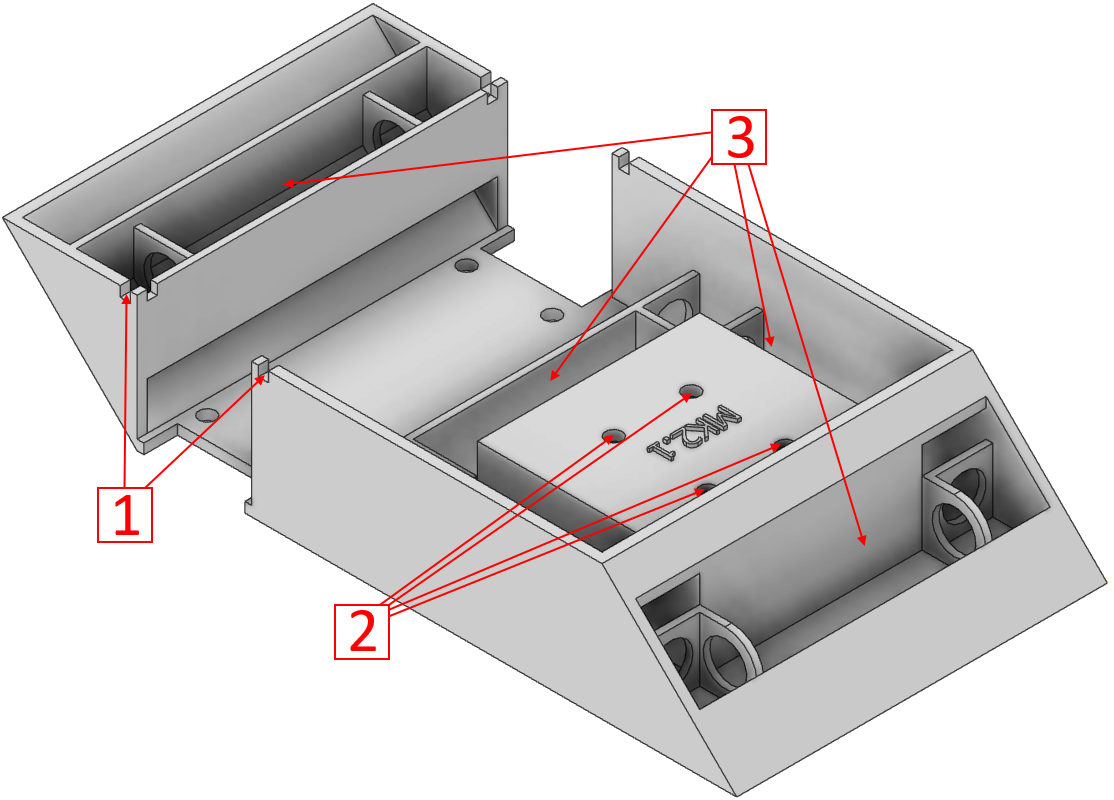
\includegraphics[scale=0.38]{images/Model3D_Rama.png}
      \label{fig:model3dramagora}
    }\qquad
    \subfloat[Widok z dołu]{
      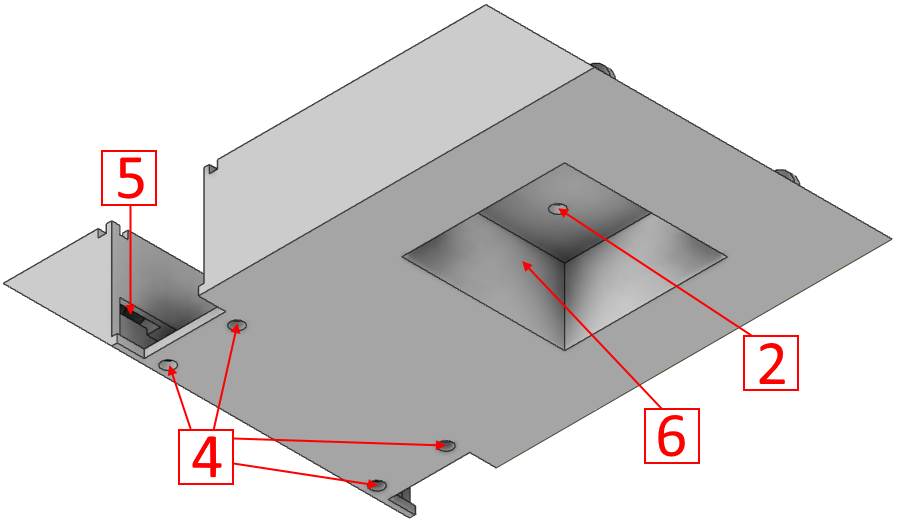
\includegraphics[scale=0.47]{images/Model3D_Rama_Spod.png}
      \label{fig:model3dramaspod}
    }
    \caption{Model 3D ramy pojazdu: a) widok z góry, b) widok z dołu}
    \label{fig:model3drama}
\end{figure}

\begin{enumerate}
    \item Uchwyty na osłony silników
    \item Otwory na śruby mocujące koło podporowe
    \item Sloty na akumulatory zasilające
    \item Otwory na śruby mocujące osłony silników
    \item Otwory na przewody akumulatorów zasilających
    \item Przestrzeń na koło podporowe
\end{enumerate}

Drugim modułem modelu 3D są osłony silników. Zakładana odległość pojazdu od ziemii wynosi 5~mm, więc wraz ze wzrostem średnicy kół konieczne jest podniesienie tylnej osi. W~przeciwnym wypadku, pojazd zacząłby podnosić się z~tylu, co spowodowałoby przy większych średnicach uderzenie przodu pojazdu o~podłoże. Model został więc stworzony tak, by zmieniać wysokość osi w razie potrzeby. Model osłony silników dla kół o~średnicy 30~mm przedstawiono na Rysunku \ref{fig:oslonasilnikow}.

\begin{figure}[!h]
    \centering
    \subfloat[Widok z góry]{
        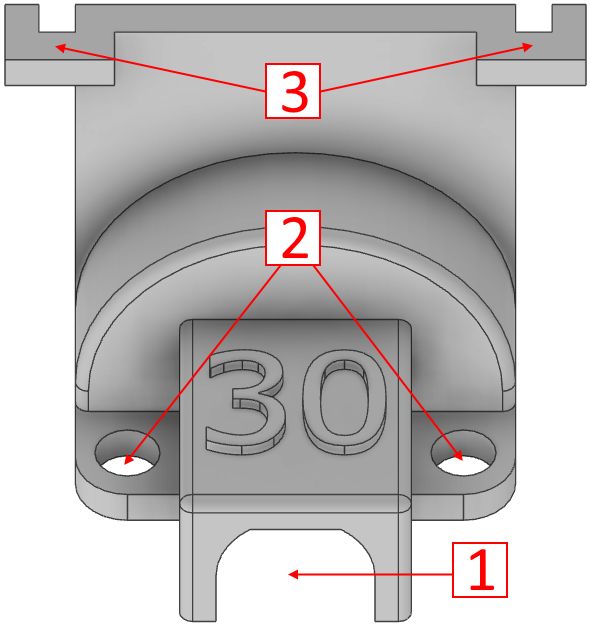
\includegraphics[scale=0.35]{images/Model3D_Oslona_1.png}
      \label{fig:moslonasilnikowgora}
    }\qquad
    \subfloat[Widok z dołu]{
      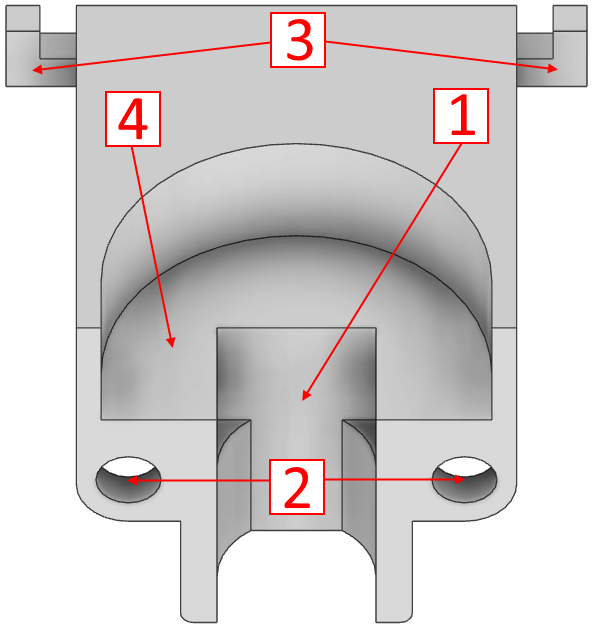
\includegraphics[scale=0.35]{images/Model3D_Oslona_2.png}
      \label{fig:oslonasilnikowspod}
    }
    \caption{Model 3D osłony silnika: a) widok z góry, b) widok z dołu}
    \label{fig:oslonasilnikow}
\end{figure}

\begin{enumerate}
    \item Przestrzeń mocowania silnika
    \item Otwory na śruby mocujące osłony silników
    \item Uchwyty przytwierdzające osłony do ramy
    \item Przestrzeń koła
\end{enumerate}

Ostatnim elementem pojazdu są koła. Podstawową wartością w~projekcie jest średnica 30~mm. Model widoczny na Rysunku \ref{fig:kolo}

\begin{figure}[!h]
    \centering
    \subfloat[Widok z góry]{
        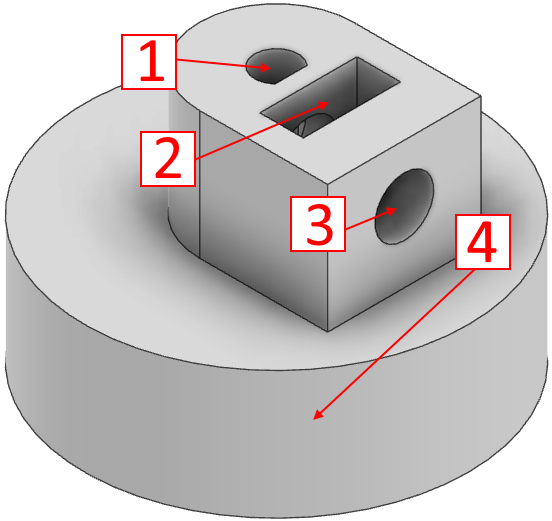
\includegraphics[scale=0.38]{images/Model3D_Kolo_1.png}
      \label{fig:kologora}
    }\qquad
    \subfloat[Widok z dołu]{
      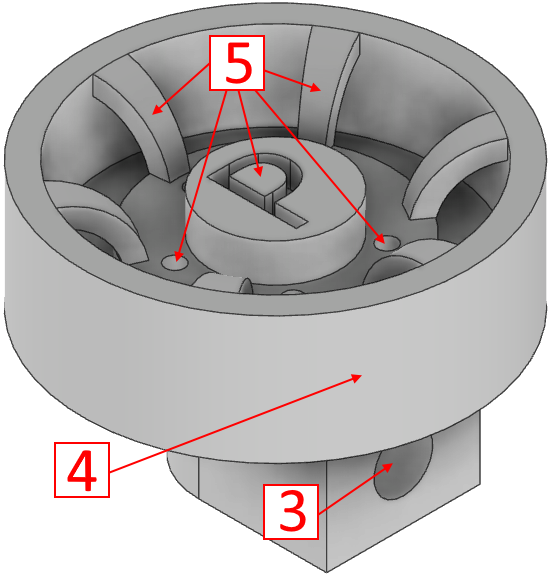
\includegraphics[scale=0.35]{images/Model3D_Kolo_2.png}
      \label{fig:kolospod}
    }
    \caption{Model 3D osłony silnika: a) widok z góry, b) widok z dołu}
    \label{fig:kolo}
\end{figure}

\begin{enumerate}
    \item Otwór wału silnika
    \item Przestrzeń nakładki śruby dociskowej
    \item Przestrzeń śruby dociskowej
    \item Koło
    \item Elementy ozdobne
\end{enumerate}

\subsection*{Elektronika}
Podstawową funkcją układu elektronicznego jest obsługa 2~silników DC. Wymaga to zastosowania elementu generującego sygnał sterujący, zasilania, oraz części przekazującej moc do silników. Jako serce układu wybrano mikrokontroler ESP32-DevKitC~V4 (Rysunek~\ref{fig:esp32}). Odpowiada on za wszystkie najważniejsze operacje: odbieranie i~wysyłanie danych po Wi-Fi, rozpoczynanie i~kończenie pomiarów, oraz generowanie sygnału sterującego. Dokładną specyfikację techniczną pominięto, ponieważ nie jest ona istotna w kontekście projektu. Została dobrana tak, by spełniała założenia projektowe (sterowanie PWM i obsługa Wi-Fi).

\begin{center}
    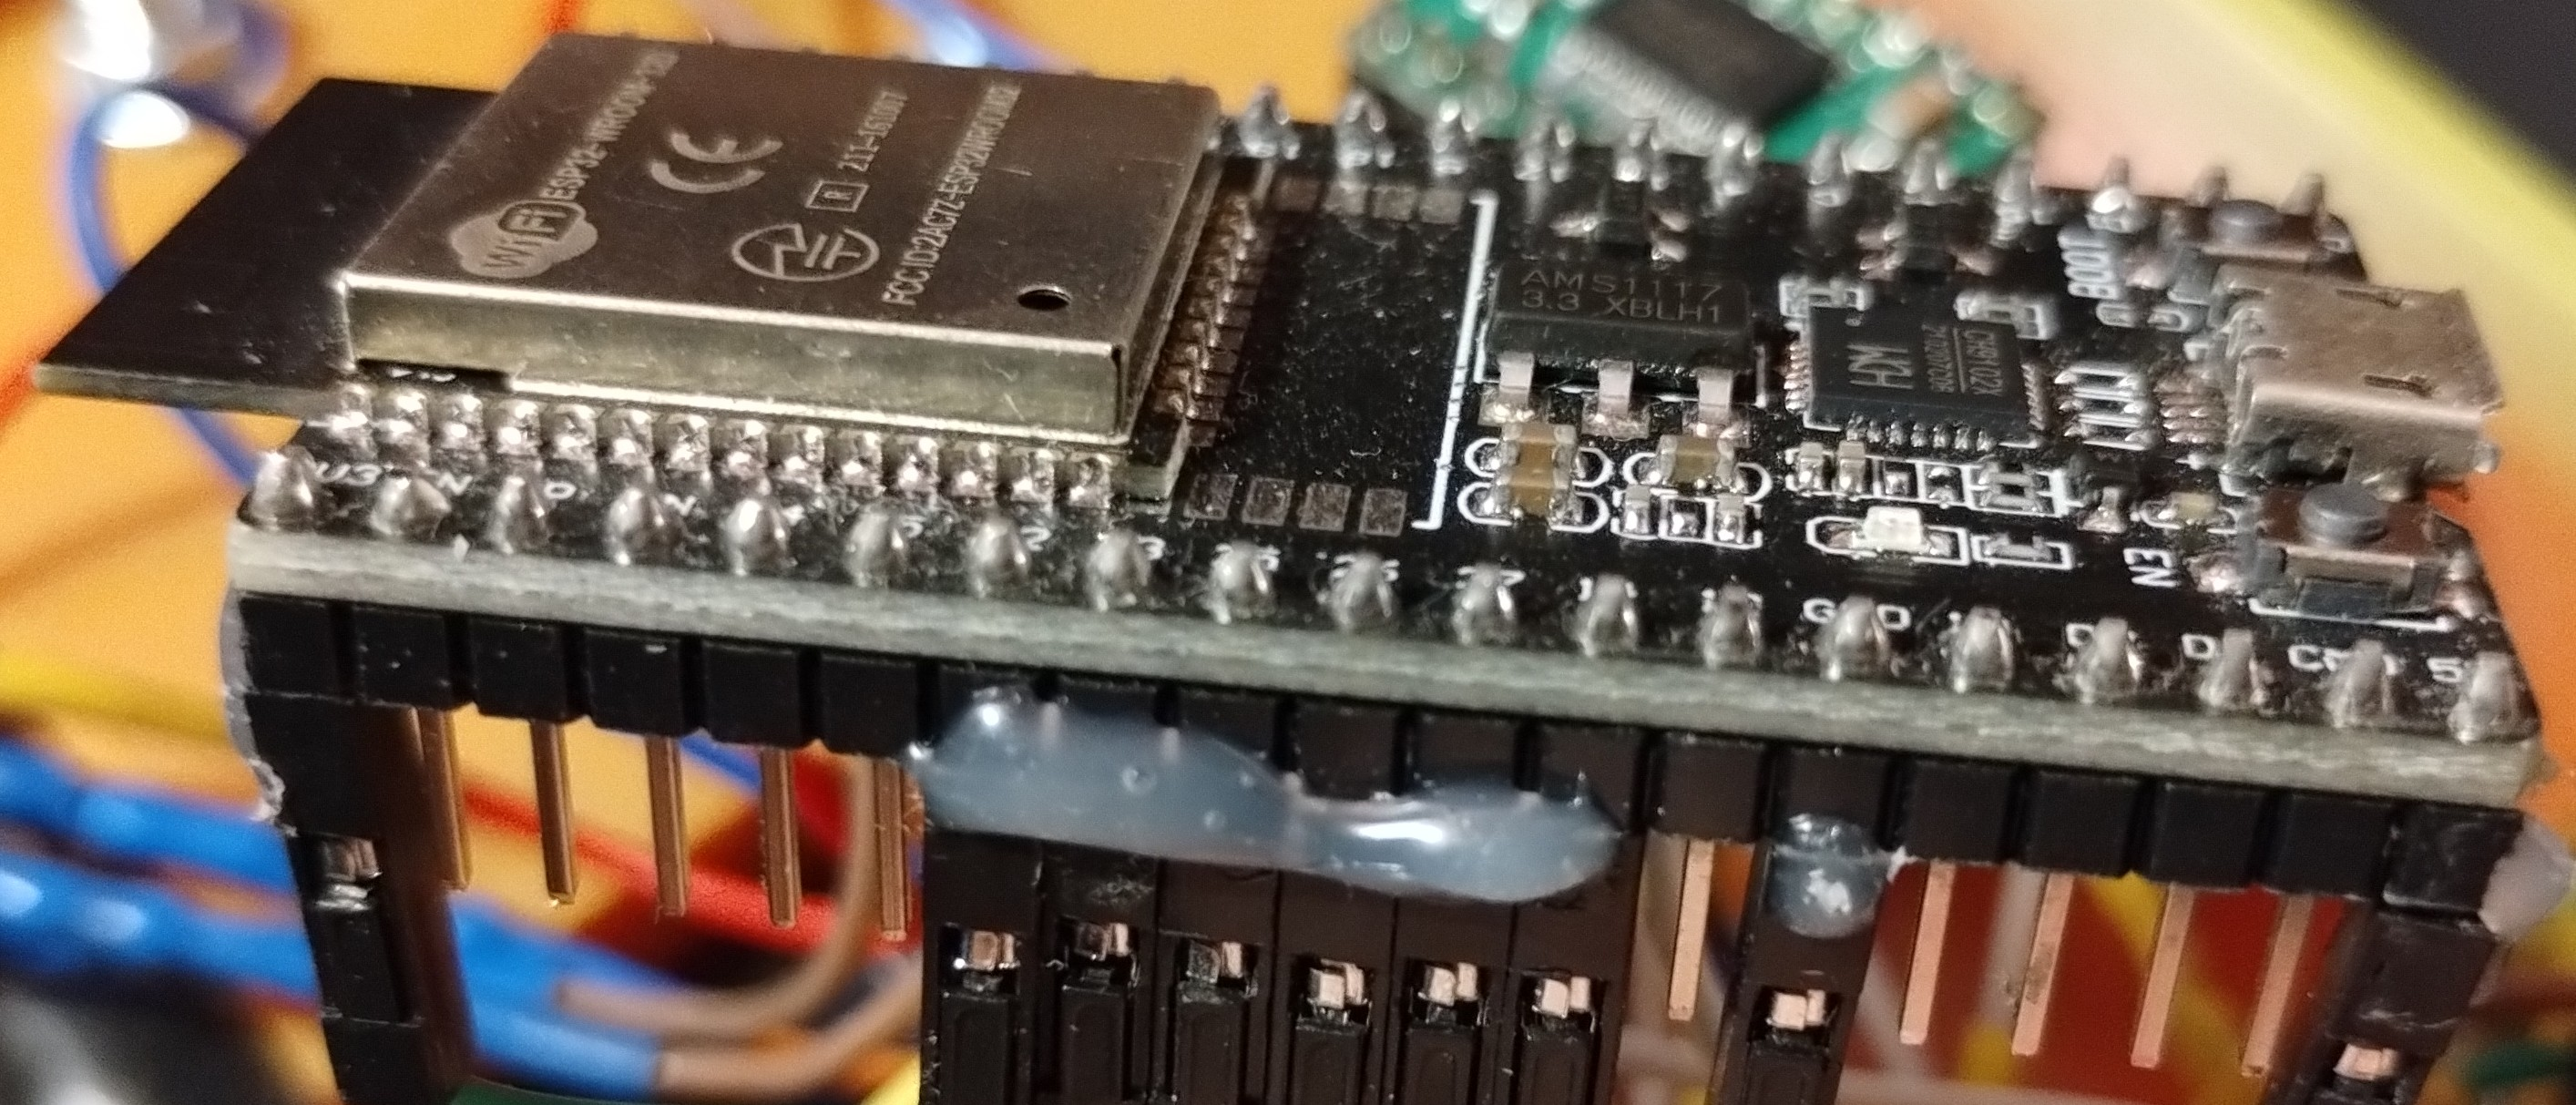
\includegraphics[scale=0.08]{images/ESP32.jpg}
    \captionof{figure}{Płytka mikrokontrolerowa ESP32-DevKitC V4}
    \label{fig:esp32}
\end{center}

Napędem są 2~silniki DC z~enkoderami magnetycznymi widoczne na Rysunku \ref{fig:motor}. Informacyjnie zamieszczono również ich specyfikację w~Tabeli \ref{tab:motor}.

\begin{center}
    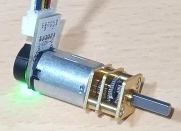
\includegraphics[scale=1]{images/Silnik.png}
    \captionof{figure}{Silnik DC z enkoderem magnetycznym (Bibliografia: \cite{bib:silnikali})}
    \label{fig:motor}
\end{center}

\begin{table}[!h]
    \begin{tabular}{|cccccc|}
    \hline
    \multicolumn{6}{|c|}{\textbf{Specyfikacja silników}} \\ \hline
    \multicolumn{1}{|c|}{\begin{tabular}[c]{@{}c@{}}Napięcie\\ zamionowe\end{tabular}} & \multicolumn{1}{c|}{12 V}  & \multicolumn{1}{c|}{\begin{tabular}[c]{@{}c@{}}Prędkość\\ znamionowa\end{tabular}}          & \multicolumn{1}{c|}{230 RPM}   & \multicolumn{1}{c|}{\begin{tabular}[c]{@{}c@{}}Prędkość na\\ biegu jałowym\end{tabular}}    & 300 RPM   \\ \hline
    \multicolumn{1}{|c|}{Przełożenie}                                                  & \multicolumn{1}{c|}{100:1} & \multicolumn{1}{c|}{\begin{tabular}[c]{@{}c@{}}Moment\\ obrotowy\\ znamionowy\end{tabular}} & \multicolumn{1}{c|}{200 g.cm}  & \multicolumn{1}{c|}{\begin{tabular}[c]{@{}c@{}}Moment\\ obrotowy\\ maksymalny\end{tabular}} & 1.6 kg.cm \\ \hline
    \multicolumn{1}{|c|}{\begin{tabular}[c]{@{}c@{}}Prąd\\ blokady\end{tabular}}       & \multicolumn{1}{c|}{0.9 A} & \multicolumn{1}{c|}{\begin{tabular}[c]{@{}c@{}}Prąd na\\ biegu jałowym\end{tabular}}        & \multicolumn{1}{c|}{$\leq$ 75 mA} & \multicolumn{1}{c|}{Prąd znamionowy}                                                        & $\leq$ 0.3 A \\ \hline
    \multicolumn{1}{|c|}{\begin{tabular}[c]{@{}c@{}}Liczba impulsów\\ enkodera na obrót\end{tabular}} & \multicolumn{1}{c|}{7}     & \multicolumn{1}{c|}{\begin{tabular}[c]{@{}c@{}}Napięcie\\ znamionowe\\ enkodera\end{tabular}} & \multicolumn{1}{c|}{\begin{tabular}[c]{@{}c@{}}3.3 V\\ do 5 V\end{tabular}} & \multicolumn{1}{c|}{\begin{tabular}[c]{@{}c@{}}Sygnał\\ wyjściowy\\ enkodera\end{tabular}}  & \begin{tabular}[c]{@{}c@{}}Cyfrowa\\ funkcja\\ kwadratowa\end{tabular} \\ \hline
    \end{tabular}
    \caption{Specyfikacja silnika DC z enkoderem magnetycznym (Bibliografia: \cite{bib:silnikali})}
\end{table}
\label{tab:motor}

Do zasilania wykorzystano akumulatory litowo-jonowe typu 18650. Ponieważ pojedynczy akumulator posiada napięcie znamionowe 3.7~V i~maksymalne 4.2~V, połączono je szeregowo w~2~grupach po 2~i~3 --- dając odpowiednio 6.4~V do 8.2~V i~10.8~V do 12.6~V --- w~celu zasilania odpowiednio ESP32 i~silników.

Zasilania nie można niestety podłączyć bezpośrednio do silników. Spowodowałoby to działanie w~trybie ciągłym na pełnej mocy, bez możliwości zmiany polaryzacji, co byłoby całkowicie sprzeczne z~założeniami projektowymi. Konieczne jest podłączenie w~taki sposób, by możliwe było przekazanie sygnału sterującego z~ESP32, oraz zmiana polaryzacji. Zastosowanie połączenia pośredniego przez samą płytkę ESP32 jest niestety niemożliwe, ponieważ nie jest w stanie ona obsłużyć tak dużych prądów. Użyto więc w~tym celu sterownika silników DC, model TB6612FNG firmy Pololu (Rysunek \ref{fig:sterownik}). Działa on na zasadzie mostka~H, umożliwiającego zmianę polaryzacji. Dzięki budowie dwukanałowej, jeden sterownik umożliwia obsługę 2~silników. Posiada również ochronę przed prądami zwrotnymi, termiczny obwód odcinający i~kondensatory filtrujące. Informacyjnie zamieszczono również jego specyfikację w~Tabeli \ref{tab:sterownik}.

\begin{center}
  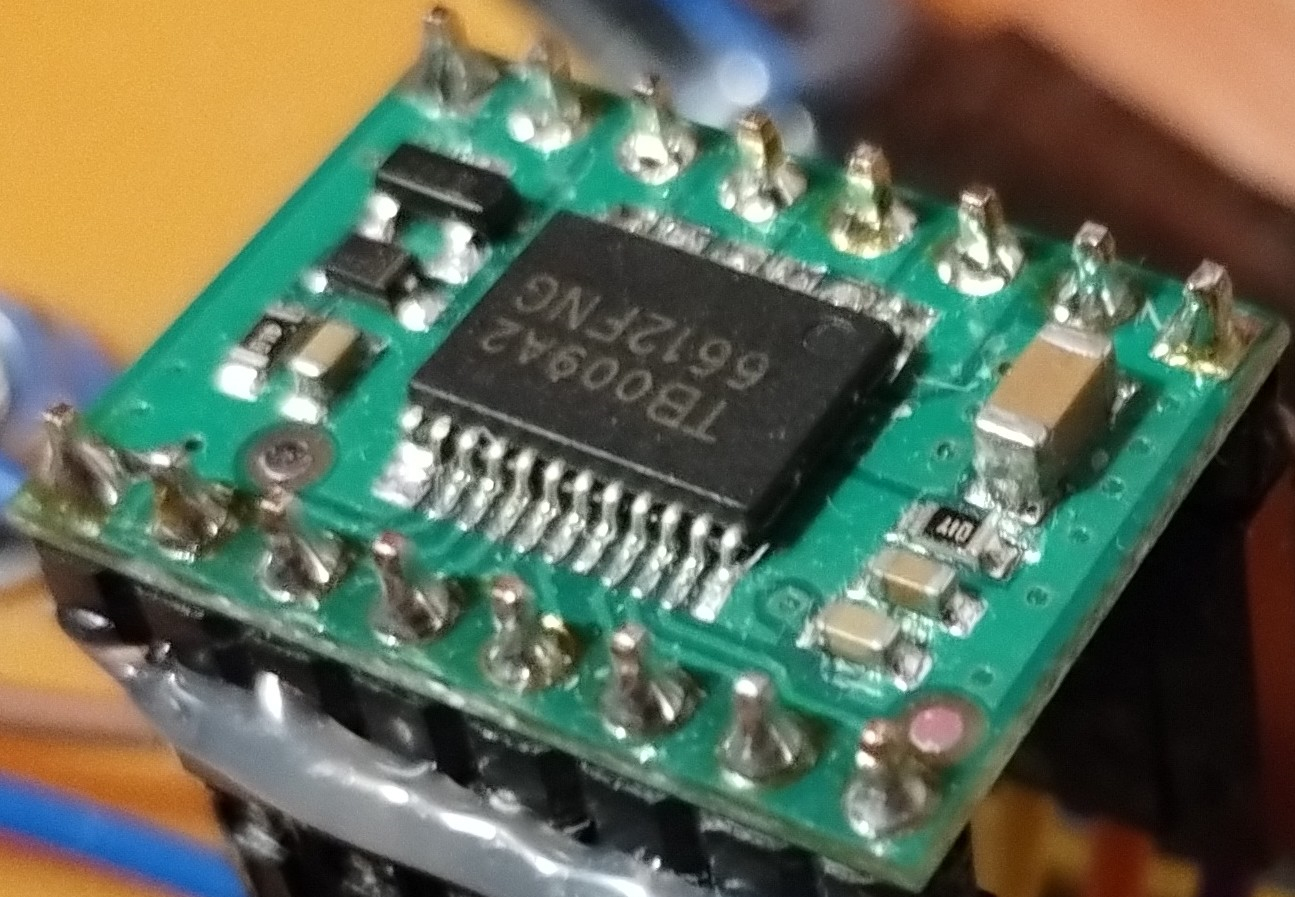
\includegraphics[scale=0.25]{images/Sterownik.jpg}
  \captionof{figure}{Sterownik silników DC TB6612FNG}
  \label{fig:sterownik}
\end{center}

\begin{table}[!h]
  \begin{tabular}{|cccccc|}
  \hline
  \multicolumn{6}{|c|}{\textbf{Specyfikacja sterownika TB6612FNG}}   \\ \hline
  \multicolumn{1}{|c|}{\begin{tabular}[c]{@{}c@{}}Zasilanie\\ silników (VMOT)\end{tabular}}        & \multicolumn{1}{c|}{\begin{tabular}[c]{@{}c@{}}4.5 V\\ do 13.5 V\end{tabular}} & \multicolumn{1}{c|}{\begin{tabular}[c]{@{}c@{}}Zasilanie układu\\ logicznego (VCC)\end{tabular}}    & \multicolumn{1}{c|}{\begin{tabular}[c]{@{}c@{}}2.7 V\\ do 5.5 V\end{tabular}} & \multicolumn{1}{c|}{\begin{tabular}[c]{@{}c@{}}Maksymalna\\ częstotliwość\\ PWM\end{tabular}} & 100 kHz \\ \hline
  \multicolumn{1}{|c|}{\begin{tabular}[c]{@{}c@{}}Ciągły prąd\\ wyjściowy\\ na kanał\end{tabular}} & \multicolumn{1}{c|}{1 A}                                                       & \multicolumn{1}{c|}{\begin{tabular}[c]{@{}c@{}}Maksymalny\\ prąd wyjściowy\\ na kanał\end{tabular}} & \multicolumn{1}{c|}{3 A}                                                      & \multicolumn{1}{c|}{\begin{tabular}[c]{@{}c@{}}Łączny ciągły\\ prąd maksymalny\end{tabular}}  & 2 A     \\ \hline
  \end{tabular}
  \caption{Specyfikacja sterownika silników DC TB6612FNG (Bibliografia: \cite{bib:sterownik})}
\end{table}
\label{tab:sterownik}

Dużym wyzwaniem okazał się dobór odpowiedniego czujnika laserowego, który z~wysoką precyzją mierzyłby dokładność przebytej odległości i~pomiarów z enkoderów. Pierwszym problemem był wybór takiego czujnika, który działałby z~odpowiednią precyzją i~dokładnością. Wymagana jest dokładność poniżej 5~mm, idealnie w~okolicach 1~mm. Drugi problem to kąt działania czujnika. Większość z~nich oferuje kąt działania w~okolicach 15$^{\circ}$ symetryczny wokół środka, dając promień 7.5$^{\circ}$. Czujnik znajdowałby się bardzo blisko podłogi, co tworzyłoby ryzyko, że utworzony przez kąt działania stożek uderzałby o~podłogę i~wykrywał ją jako przeszkodę, lub wykrywał inne niepożądane poboczne obiekty, niwelując tym samym użyteczność otrzymanych pomiarów. Dalmierze oferujące pomiar punktowy lub bliski punktowemu posiadają znaczne wymiary, niską kompatybilność z~elektroniką hobbystyczną (ESP32), dużą masę, i/lub wysoką cenę. Istnieją dalmierze hobbystyczne które idealnie nadawałyby się jako element pomiarowy, lecz ich dystans pomiarowy jest niewielki i wynosi kilka do kilkudziesięciu centymetrów. Rozwiązaniem alternatywnym byłoby wykorzystanie systemu LIDAR (ang.~\english{Light Detection and Ranging}), który umożliwia nie tylko punktowy pomiar odległości, lecz mapowanie danego obszaru wykorzystując technologię czujników laserowych. Istnieją modele spełniające założenia projektowe i~mieszczące się w sensownym budżecie, jednak ich wykorzystanie wymagałoby znacznych nakładów czasowych w~celu nauki sprzętu, zaprogramowania odpowiednich funkcjonalności, a~następnie testów. Z~tego powodu zdecydowano o~porzuceniu idei pomiaru laserowego i~zamiast tego wykorzystanie pomiaru manualnego z~pomocą dostępnego powszechnie przymiaru liniowego.

Enkodery magnetyczne zostały zapewnione w~silnikach napędowych --- stanowią wspólną całość, wymagane jest jedynie ich odpowiednie podłączenie w postaci przewodów zasilających i~sygnałowych. Do sygnalizowania stanu oprogramowania ESP32, czyli aktualnego stanu w~jakim znajduje się układ, założono instalację LED oraz głośnika. Po zamontowaniu LED w~układzie i~przetestowaniu rozwiązania, okazało się, że jest ono wystarczające do spełnienia założonego celu. Tym samym, montaż głośnika stał się zbędny i~usunięto go z~założeń projektowych. Przełączniki źródeł prądowych zamontowano szeregowo przy akumulatorach zasilających, w~postaci normalnie otwartych przycisków bistabilnych.

LEDy po podłączeniu standardowego napięcia zasilającego --- w~tym przypadku zakres od 2~V do 3.3~V, w~zależności od koloru diody --- doświadczają przepływu prądu znacznie większego, niż prąd nominalny (dla wykorzystanych diod 22~mA). Z~tego powodu, w~celach ochronnych stosuje się rezystory obniżające wartość przepływającego prądu. W~większości przypadków wartość rezystora dobiera się stosując prawo Ohma, dla rzeczywistych układów biorąc również pod uwagę spadek napięcia na diodzie, wynoszący około 0.7~V. W~tym projekcie nie ma jednak potrzeby stosowania obliczeń, ponieważ gotowe wartości rezystorów zostały podane przez producenta. 100$\Omega$ dla diody czerwonej, 82$\Omega$ dla zielonej i~47$\Omega$ dla niebieskiej. Z~powodu braku dostępności rezystora 82$\Omega$, połączono szeregowo 3~rezystory o~wartościach 10$\Omega$, 22$\Omega$ i~47$\Omega$, dając łącznie 79$\Omega$. Podłączenie wykonano w~układzie wspólnej katody.

Do zabezpieczenia układu wykorzystano popularne bezpieczniki topikowe. Włączone zostały w~układ szeregowo przy akumulatorach zasilających. Jako że zarówno sterownik jak i~ESP32 posiadają wewnętrzne zabezpieczenia nadprądowe do pewnego progu, zadaniem bezpieczników nie jest ograniczenie prądu poniżej konkretnych wartości, lecz zabezpieczenie przed zwarciem. Prąd zwarciowy dla akumulatorów typu 18650 wynosi około 30~A do 40~A, czego żaden z układów ani przewodów by nie wytrzymały. Dlatego wartości zostały dobrane arbitralnie i wynoszą 0.1~A i 0.25~A dla 230~V, dając odpowiednio 23~W i 57.5~W. Są to wartości wystarczające by umożliwić układowi swobodne działanie, a jednocześnie zabezpieczyć przed zwarciem.

Pełny schemat układu elektronicznego przedstawiono na Rysunku \ref{fig:schematelektryczny}

\begin{center}
  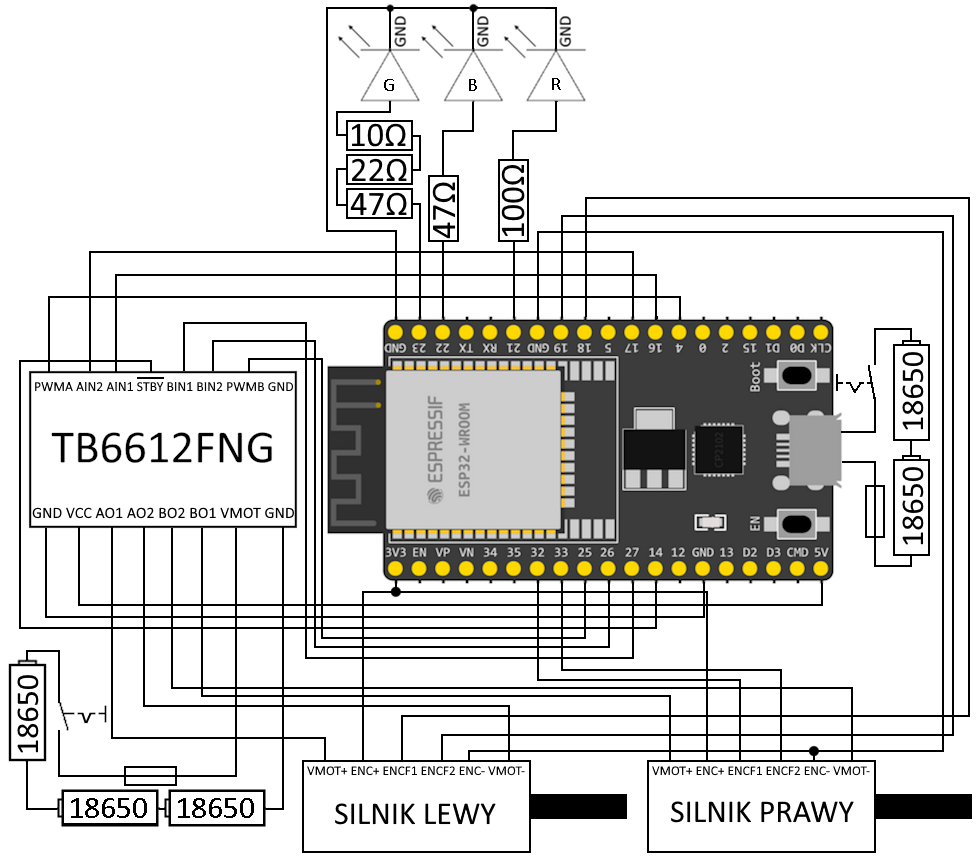
\includegraphics[scale=0.61]{images/Schemat_elektryczny.png}
  \captionof{figure}{Schemat układu elektronicznego}
  \label{fig:schematelektryczny}
\end{center}

Oznaczenia silników:
\begin{enumerate}
  \item VMOT+ --- zasilanie silników
  \item ENC+ --- zasilanie enkoderów
  \item ENCF1, ENCF2 --- sygnały zwrotne enkoderów
  \item ENC-- --- uziemienie enkoderów
  \item VMOT-- --- uziemienie silników
\end{enumerate}

\newpage % bo te 2 smutne linijki na końcu brzydko wyglądają

Oznaczenia sterownika:
\begin{enumerate}
  \item PWMA --- wejście sygnału PWM lewego silnika
  \item AIN2 --- wejście polaryzacji lewego silnika 2
  \item AIN1 --- wejście polaryzacji lewego silnika 1
  \item STBY --- tryb postoju/oszczędzania energii (ang.~\english{standby}), aktywacja sygnałem niskim
  \item BIN1 --- wejście polaryzacji prawego silnika 1
  \item BIN2 --- wejście polaryzacji prawego silnika 2
  \item PWMA --- wejście sygnału PWM prawego silnika
  \item GND --- uziemienie, wszystkie 3~piny są połączone
  \item VCC --- zasilanie układu logicznego sterownika
  \item AO1 --- wyjście zasilające lewego silnika 1
  \item AO2 --- wyjście zasilające lewego silnika 2
  \item BO2 --- wyjście zasilające prawego silnika 2
  \item BO1 --- wyjście zasilające prawego silnika 1
  \item VMOT --- wejście zasilające silników
\end{enumerate}

Na Rysunkach \ref{fig:pojazdgora}, \ref{fig:pojazddol} pokazano końcowy efekt, po złożeniu ze sobą wszystkich komponentów. Niestety w trakcie wykonywania zdjęć, przewód zasilający płytkę ESP32 uległ uszkodzeniu przez zmęczenie materiałowe. Jest to uszkodzenie o niskim priorytecie, którego naprawa nie przyniosłaby większych korzyści. Z tego powodu pozostałe badania eksperymentalne i samo nagranie z działania zostały wykonane na zasilaniu ze źródła zewnętrznego, banku energii (ang.\english{power bank}). 

\begin{center}
  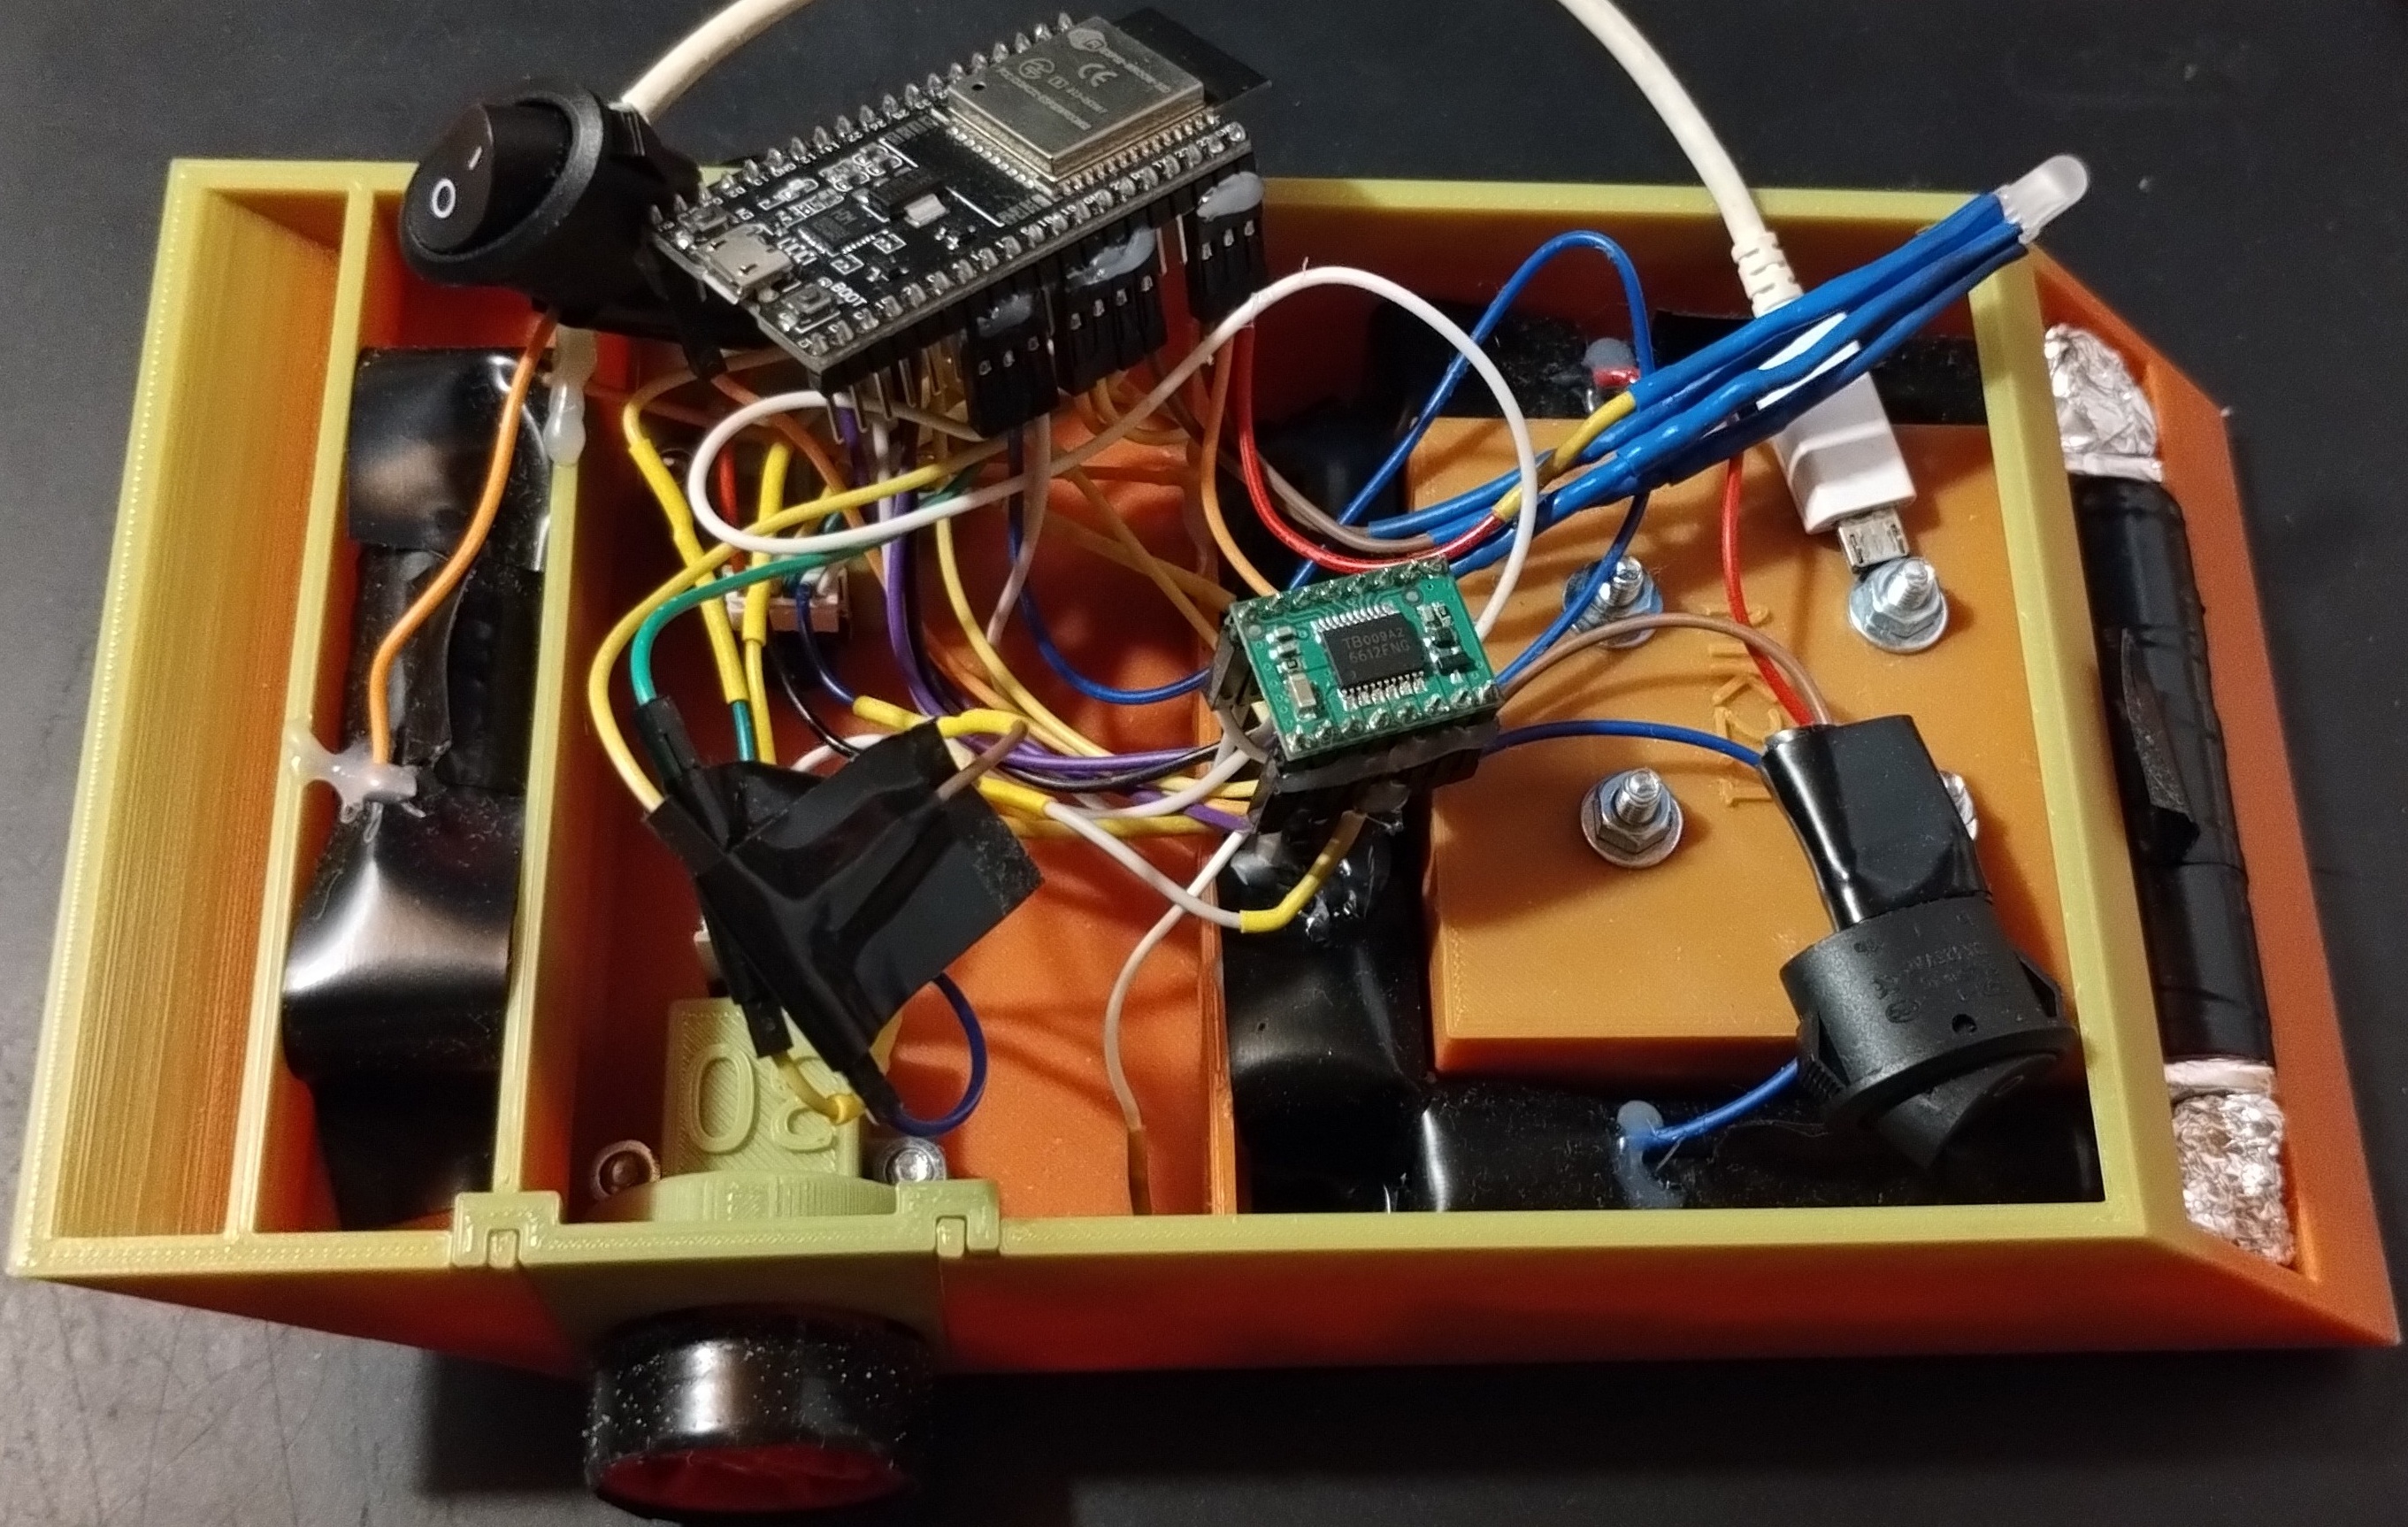
\includegraphics[scale=0.21]{images/Pojazd_Gora.jpg}
  \captionof{figure}{Zdjęcie pojazdu z góry}
  \label{fig:pojazdgora}
\end{center}

\begin{center}
  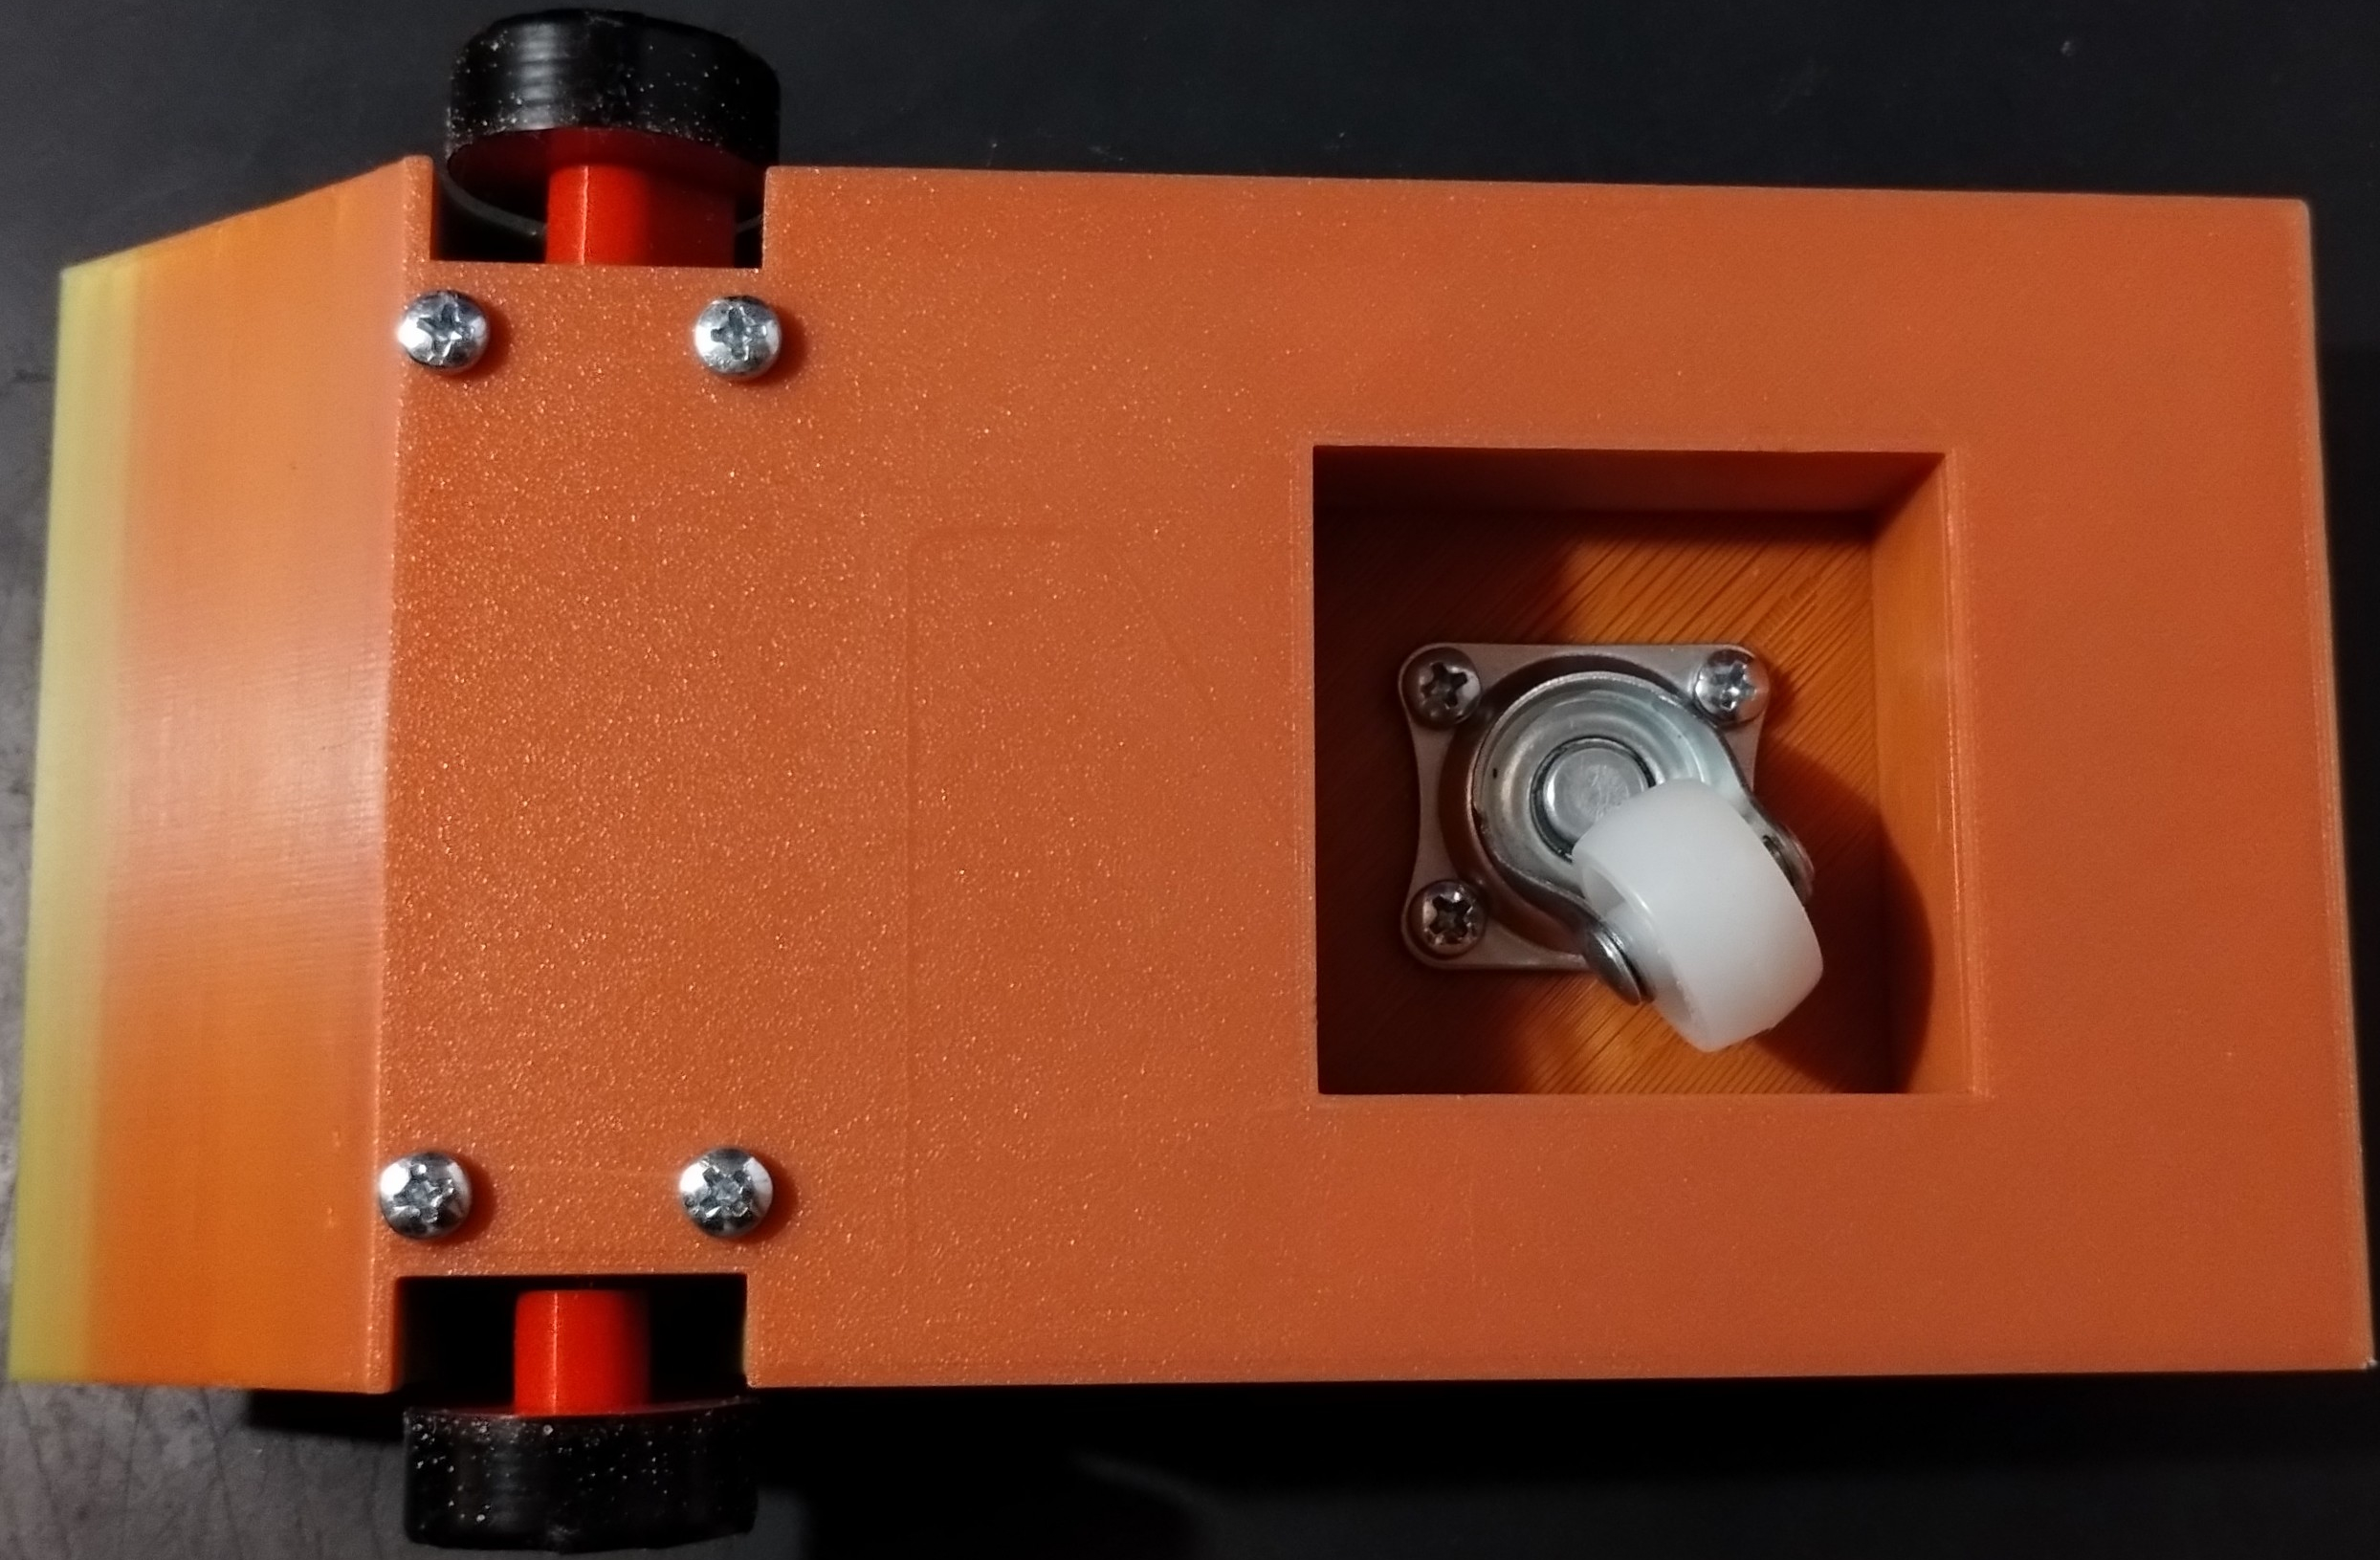
\includegraphics[scale=0.23]{images/Pojazd_Dol.jpg}
  \captionof{figure}{Zdjęcie pojazdu z dołu}
  \label{fig:pojazddol}
\end{center}

\subsection*{Oprogramowanie}
Oprogramowanie pojazdu podzielone zostało na kilka modułów, każdy z~nich umieszczono w~osobnym pliku~.cpp. Poszczególne moduły działają na osobnych zadaniach (ang. \english{task}), w~zależności od potrzeb niektóre na więcej niż jednym. ESP32 posiada 2~rdzenie, o~numeracji 0~i~1. Rdzeń pierwszy odpowiada domyślnie za obsługę modułów fizycznych, takich jak Wi-Fi i~Bluetooth, zaś drugi za wykonanie reszty kodu. Aby zapewnić enkoderom możliwie najwięcej czasu procesora i~największą ilość przerwań, moduły odpowiadające za regulator (i~tym samym enkodery) umieszczono na rdzeniu pierwszym, zaś całą resztę na rdzeniu zerowym. Poniżej umieszczono krótkie opisy poszczególnych modułów, szczegółowe opisy funkcjonalności znajdują się w odpowiedniej dla danego modułu sekcji.

\begin{itemize}
  \item Moduł główny --- zawiera jedynie funkcję startową \textit{app{\_}main}, wywołującą pozostałe moduły (dlatego nie posiada osobnej sekcji)
  \item Moduł łączności --- obsługuje utrzymywnaie połączenia Wi-Fi, oraz serwera i~klienta UDP
  \item Moduł regulatora --- przetwarza pulsy otrzymane z enkoderów, oraz oblicza sygnały sterujące
  \item Moduł procesora pakietów --- odczytuje zawartość ramek z~pakietów UDP i~zapisuje ich zawartość
  \item Moduł konfiguracyjny --- przechowuje w jednym miejscu wszystkie najważniejsze zmienne konfiguracyjne systemu
\end{itemize}

\subsubsection*{Moduł łączności}
Po wywołaniu z~modułu głównego, moduł łączności rozpoczyna 3~zadania: podtrzymywania połączenia Wi-Fi, serwera UDP i~klienta UDP. Zadanie podtrzymania Wi-Fi uruchamia połączenie z~siecią, a~następnie przechodzi do nieskończonej pętli sprawdzającej czy połączenie nie zostało przerwane (Źródło: \ref{lst:conwhiletrue}). Jeśli zostało przerwane, podejmowane są odpowiednie czynności --- zmiana koloru LED na czerwony, oraz zatrzymanie pomiaru (a~co za tym idzie, wyłączenie silników), jeśli był on w~trakcie. Wykrywanie przerwania/wznowienia połączenia następuje poprzez obsługę zdarzeń (ang. \english{event handlers}) platformy (ang. \english{framework}) ESP-IDF.

Klient UDP tworzy gniazdo (ang. \english{socket}) z przypisanym adresem IP i~portem, a~po czym również wchodzi w~nieskończoną pętlę wysyłającą pakiety (Źródło: \ref{lst:udpclientwhiletrue}). Ponieważ wysyłanie pakietów bez przerwy w~nieskończonej pętli byłoby wysoce nieefektywne (na przykład w~przypadku braku pakietów do wysłania), dlatego po każdej pętli zadanie jest zatrzymywane i~wybudzane z~powrotem zewnętrznie przez inne zadanie, gdy pojawi się pakiet do wysłania.

Analogicznie działa zadanie serwera UDP odbierający pakiety, z~tą różnicą, że przyjmuje pakiety od dowolnego adresu IP, oraz działa w~ciągłej pętli w~odstępie zdefiniowanym w~pliku konfiguracyjnym (domyślnie 50~ms).

\subsection*{Moduł regulatora}
Najważniejszy moduł oprogramowania ESP32. Odczytuje, przetwarza i~zapisuje liczbę pulsów enkodera, a~następnie na ich podstawie oblicza sygnały sterujące. Obsługa enkoderów została stworzona z~wykorzystaniem dodatkowych komponentów platformy otwartoźródłowej ESP-IDF (Bibliografia: \cite{bib:espidfcomponents}).

W~pierwszej kolejności wywoływane są funkcje konfiguracyjne pinów, konfigurowane generatory sygnału PWM dla częstotliwości 25 kHz, oraz tworzone zadanie obsługujące pozostałą część kodu. Zadanie to uruchamia następnie zegar cyklicznie (co 50 ms) wywołujący funkcję obsługującą odczyt enkoderów oraz wywołującą regulator. Działanie zegara cyklicznego jest zasadniczo identyczne jak nieskończonej pętli, z~tą różnicą, że działa na przerwaniach, gwarantując tym samym stały odstęp czasowy między kolejnymi wywołaniami.

Wyrównywanie pozycji silników wykonać można na kilka różnych sposobów. W~tym projekcie wykorzystano model "prowadzący-śledzący" (ang. \english{leader-follower}). W~modelu tym, jeden z~silników przyjmuje rolę prowadzącego, tym samym posiada w~sygnale sterującym tylko jedną, niezależną część, której zadaniem jest doprowadzenie pozycji absolutnej silnika do wartości zadanej. Drugi silnik, będący śledzącym, posiada 2~części sygnału sterującego --- niezależną oraz zależną. Część niezależna ma identyczne działanie, jak w~przypadku silnika prowadzącego. Zaś część zależna odpowiada za dociągnięcie błędu między silnikiem prowadzącym a~śledzącym do~0. Funkcje silników zostały wybrane arbitralnie przez autora pracy --- silnikiem \textbf{prowadzącym} jest silnik \textbf{prawy}, a~silnikiem \textit{śledzącym} jest silnik \textit{lewy}.

Każda z~części sygnału sterującego posiada własny, osobno strojony, regulator PID. Silnik prawy posiada 1~część sygnału, silnik lewy 2~części, dając łącznie 3~regulatory PID. W~dalszej części pracy, regulatory te będą nazywane dla ułatwienia \textit{lewym}, \textit{prawym}, oraz \textit{synchronizującym}.

Z~powodu wysokiej istotności tej częsci kodu, zostanie ona szczegółowo przeanalizowana i~wyjaśniona. Kod jest możliwy do wglądu w~Źródle \ref{lst:petlaregulatora}. Zaczynając od linijki 90, czyli deklaracji funkcji, widać że przyjmuje ona argument typu \english{void}. Dodanie argumentu jest wymagane przez zegar cykliczny, jednak nie jest on w~żaden sposób wykorzystany. W~linijkach 91-92 wywoływana jest funkcja platformy ESP-IDF odczytująca aktualną pozycję absolutną wałów silników względem ich pozycji startowej. Sama pozycja startowa (położenie kątowe) jest nieistotne, ważna jest jedynie odległość od niej. Linijki 93-94 odpowiadają za obliczenie ilości impulsów od ostatniej pętli, a~95-96 zapisują aktualną pozycję absolutną jako poprzednią (wzlędem następnej pętli). Po odczytaniu enkoderów, w~linijce 98~wybudzany jest klient UDP w~celu wysłania zmierzonych danych.

W liniach 100-107 obliczane są wartości błędów, a~następnie sygnałów sterujących. Najpierw dla silnika prowadzącego, następnie dla śledzącego, na końcu synchronizującego. Równanie \ref{eq:error} ogólne uchybu (błędu) dla $i$-tej próbki zapisano poniżej.

\begin{equation}\label{eq:error}
  e(i)=w(i)-y(i)
\end{equation}

Dla silnika prowadzącego (linijka 100) wartością zadaną jest położenie absolutne wału silnika wyrażone liczbą pulsów, zaś wyjściem aktualna liczba pulsów, co odpowiada równaniu~\ref{eq:error}. Tak samo wygląda równanie niezależne dla silnika śledzącego, z~tą różnicą, że uwzględniony zostaje przeciwny kierunek obrotów silnika. Dzieje się tak, ponieważ silniki są fizycznie obrócone do siebie pod kątem 180$^{\circ}$. Zwrot obrotów deklarowany jest binarnie (0~lub~1), silniki będąc tak samo orientowane fizycznie posiadają ten sam zwrot, jednak dla obrotu o~180$^{\circ}$ należy zmienić deklarowany zwrot obrotów silnika, by uzyskać ten sam zwrot jazdy. Wyjście układu przyjmuje wtedy wartość ujemną, a~zmodyfikowane Równanie \ref{eq:errorfollower} pokazano poniżej. Tylko z~pozoru jest to sprzężenie dodatnie, ponieważ wartość y~jest ujemna.

\begin{equation}\label{eq:errorfollower}
  e(i)=w(i)+y(i)
\end{equation}

Kolejna modyfikacja następuje dla sygnału zależnego silnika śledzącego. Wartość zadana w~równaniu \ref{eq:errorfollower} zostaje zmieniona z~położenia absolutnego wału silnika, na aktualną liczbę pulsów silnika prowadzącego, dociągając błąd między położeniem silnika śledzącego a~prowadzącego do~0.

Po obliczeniu błędu, należy obliczyć wartość sygnału sterującego regulatorami PID. Równanie \ref{eq:pidregsignals} przedstawia ogólną postać dyskretną regulatora PID. W~Źródle \ref{lst:regulator} (Bibliografia: \cite{bib:espidfcomponents}\cite{bib:instrukcjalabyuapid}) wykorzystano postać niezależną regulatora PID (Równanie \ref{eq:pidreg}).

\begin{equation}\label{eq:pidregsignals}
  u(i)=u\textsubscript{P}(i)+u\textsubscript{I}(i)+u\textsubscript{D}i
\end{equation}

\begin{equation}\label{eq:pidreg}
  u(i)=k\textsubscript{P}e(i)+k\textsubscript{I}\sum_{j=0}^{i}e(j)+k\textsubscript{D}(e(i)-e(i-1))
\end{equation}

W linii 73 (Źródło \ref{lst:regulator}) sumowany jest uchyb. Aby wyeliminować zjawisko nawijania błędu (ang. \english{windup}) spowodowane sumowaniem błędu w~kolejnych próbkach do zbyt dużych wartości, co może powodować dominację sygnału całkującego nad proporcjonalnym i~różniczkującym, a~także opóźnić odpowiedź na zmianę wartości zadanej, zastosowano mechanizm zapobiegający (ang. \english{anti-windup}) w~postaci ograniczenia całkowania. Przedział został wyznaczony eksperymentalnie wspomagając się charakterystyką statyczną (Rysunek \ref{fig:charstatjalowy}) i~wygląda następująco: $EI \in \left<-100; 100\right>$, gdzie $EI$ to suma błędu (ang. \english{Error Integral}). Ograniczenie widoczne jest w liniach 74-75.

Następnie wyjście z~regulatora ograniczane jest do zakresu $u \in \left<-u\textsubscript{max}; u\textsubscript{max}\right>$. $u\textsubscript{max}$~wyznaczono na podstawie charakterystyki statycznej (Rysunek \ref{fig:charstatjalowy}). Widoczne jest na niej, że maksymalną wartością dla jednej pętli dla pełnej mocy jest liczba w~przedziale $\left<500; 600\right>$, eksperymentalnie wyznaczono jej wartość na $p\textsubscript{max}=571$. Biorąc pod uwagę dodanie obciążenia z~lekkim zapasem, wyznaczono maksymalną dozwoloną liczbę pulsów na pętlę na 400. W~pliku konfiguracyjnym (Config.cpp), zapisano limit w~postaci $u\textsubscript{max}=100\alpha$, gdzie $\alpha$~to współczynnik w~przedziale $\left<1; \frac{p\textsubscript{max}}{100}\right>$. Technicznie możliwa jest wartość $\alpha$~również w~przedziale $\left<0; 1\right)$, jednak nie ma ona sensu z~inżynierskiego punktu widzenia --- silnik będzie obracał na bardzo niskich obrotach, a~po dołożeniu obciążenia istnieje ryzyko, że nie pokona oporu statycznego, tym samym nie ruszając z~miejsca.

Na końcu (linijka 85), aktualna wartość błędu zapisywana jest do obliczenia składowej różniczkowej sygnału w~następnej pętli, a~aktualna wartość sygnału zwracana przez funkcję (linijka 87).

Wracając do kodu pętli (Źródło \ref{lst:petlaregulatora}), po otrzymaniu wartości sygnału ze wszystkich 3~regulatorów PID, następuje jego przetworzenie przed wysłaniem na sterownik. W~liniach 109-110 składowa zależna i~niezależna sygnału sterującego silnika śledzącego są sumowane, a~następnie ich suma ponownie ograniczana do $u\textsubscript{max}$.

W następnym kroku (linie 115-116), otrzymany wynik zamieniany jest na wartość procentową (Równanie \ref{eq:signaltopercent}), ponieważ taką przyjmuje jako argument wykorzystany generator sygnału PWM.

\begin{equation}\label{eq:signaltopercent}
  u(i)=u(i)(100 / p\textsubscript{max})
\end{equation}

Ostatnim krokiem przetworzenia sygnału sterującego jest ograniczenie go do wartości zadeklarowanej przez użytkownika w~aplikacji (linie 115-116), mnożąc go przez pożądaną wartość. Na przykład, dla 70\%~mocy natępuje mnożenie razy~0.7. Aby zapewnić silnikowi śledzącemu odrobinę zapasu mocy w razie potrzeby, moc silnika prowadzącego jest dodatkowo zmniejszana o~10\%.

Przed wysłaniem pożądanej wartości do generatora PWM, konieczne jest określenie zwrotu obrotu silników. Dzieje się to w~liniach 118-128 na podstawie znaku aktualnej wartości błędu. Po tej czynności, wartość sygnału zostaje wysłana do generatora PWM (linie 130-131), który generuje sygnał i~wysyła go na sterownik.

\subsection*{Moduł procesora pakietów}
Jest to moduł zawierający 3 funkcje --- przetwarzającą ramkę, sprawdzającą klucz i~sprawdzającą wartość. Funkcja przetwarzająca ramkę jest wywoływana z~modułu łączności po każdym odebranym pakiecie UDP. Funkcja ta na początku wywołuje funkcję sprawdzającą klucz. Jest to prosty mechanizm zabezpieczający przed odczytywaniem niepotrzebnych pakietów. Jako że ESP32 może otrzymywać dowolne pakiety z~dowolnego pakietu, w~trakcie testów kilka razy zdarzyło się, że funkcja otrzymywała wiadomości inne niż pożądane, z~którymi sobie nie radziła. Jeśli ramka nie zawiera klucza, funkcja kończy działanie. Zmiana klucza możliwa jest w pliku konfiguracyjnym, jednak trzeba pamiętać o zmianie jego długości w odpowiedniej pętli odczytującej. Ponieważ nie została zaimplementowana żadna metoda szyfrowania, zmiana klucza ramki w żaden sposób nie zwiększa cyberbezpieczeństwa. Służy on jedynie do identyfikacji źródła wiadomości.

Jeśli zawiera klucz, rozpoczyna odczytywanie danych z~ramki. Ma ona postać \textit{KLUCZA1B2C3D4Z}. Każda litera następująca po kluczu oznacza inną zmienną. Dla przykładu \textit{A}~oznacza wartość zadaną, \textit{B}~wzmocnienie $K\textsubscript{P}$~regulatora PID silnika śledzącego, itp. W~momencie pisania tego tekstu, ramka sięga litery \textit{K}.~Po wykryciu litery, ramka przekazywana jest do funkcji odczytującej następującą po niej wartość. Po zwróceniu wartości, zapisywana jest ona do odpowiedniej zmiennej. Proces ten trwa do napotkania litery \textit{Z},~oznaczającej koniec ramki. Osobnym oznaczeniem jest literka \textit{Q} oznaczająca wyście (ang. \english{quit}), która nie posiada żadnej wartości, lecz informuje program o zakończeniu pomiaru. 

\subsection*{Moduł konfiguracyjny}
Jego istnienie nie jest technicznie wymagane do działania programu, lecz znacząco zwiększa komfort użytkowania. Zawiera najważniejsze zmienne i~instancje struktur programu, tak, by możliwa była wygodna zmiana ich wartości w~dowolnym momencie, bez konieczności zmiany wszystkich wystąpień w~kodzie. Zmniejsza to również ryzyko pomyłek przez przypadkowe pominięcie wystąpienia danej zmiennej.

\section{Oprogramowanie pomocnicze}
Do wykonania projektu koniecznych było kilka dodatkowych narzędzi pomocniczych.

\subsection*{Aplikacja}
Głównym z~narzędzi jest aplikacja na system Android, przesyłająca dane użytkownika do systemu. Ponieważ została utworzona w~internetowym kreatorze, autorowi nie jest znany jej dokładny kod. Paczka plików aplikacji przed kompilacją jest dołączona do pracy jako załącznik. Na Rysunku \ref{fig:aplikacja} pokazano wygląd aplikacji po uruchomieniu, z~domyślnymi wartościami.

\begin{center}
  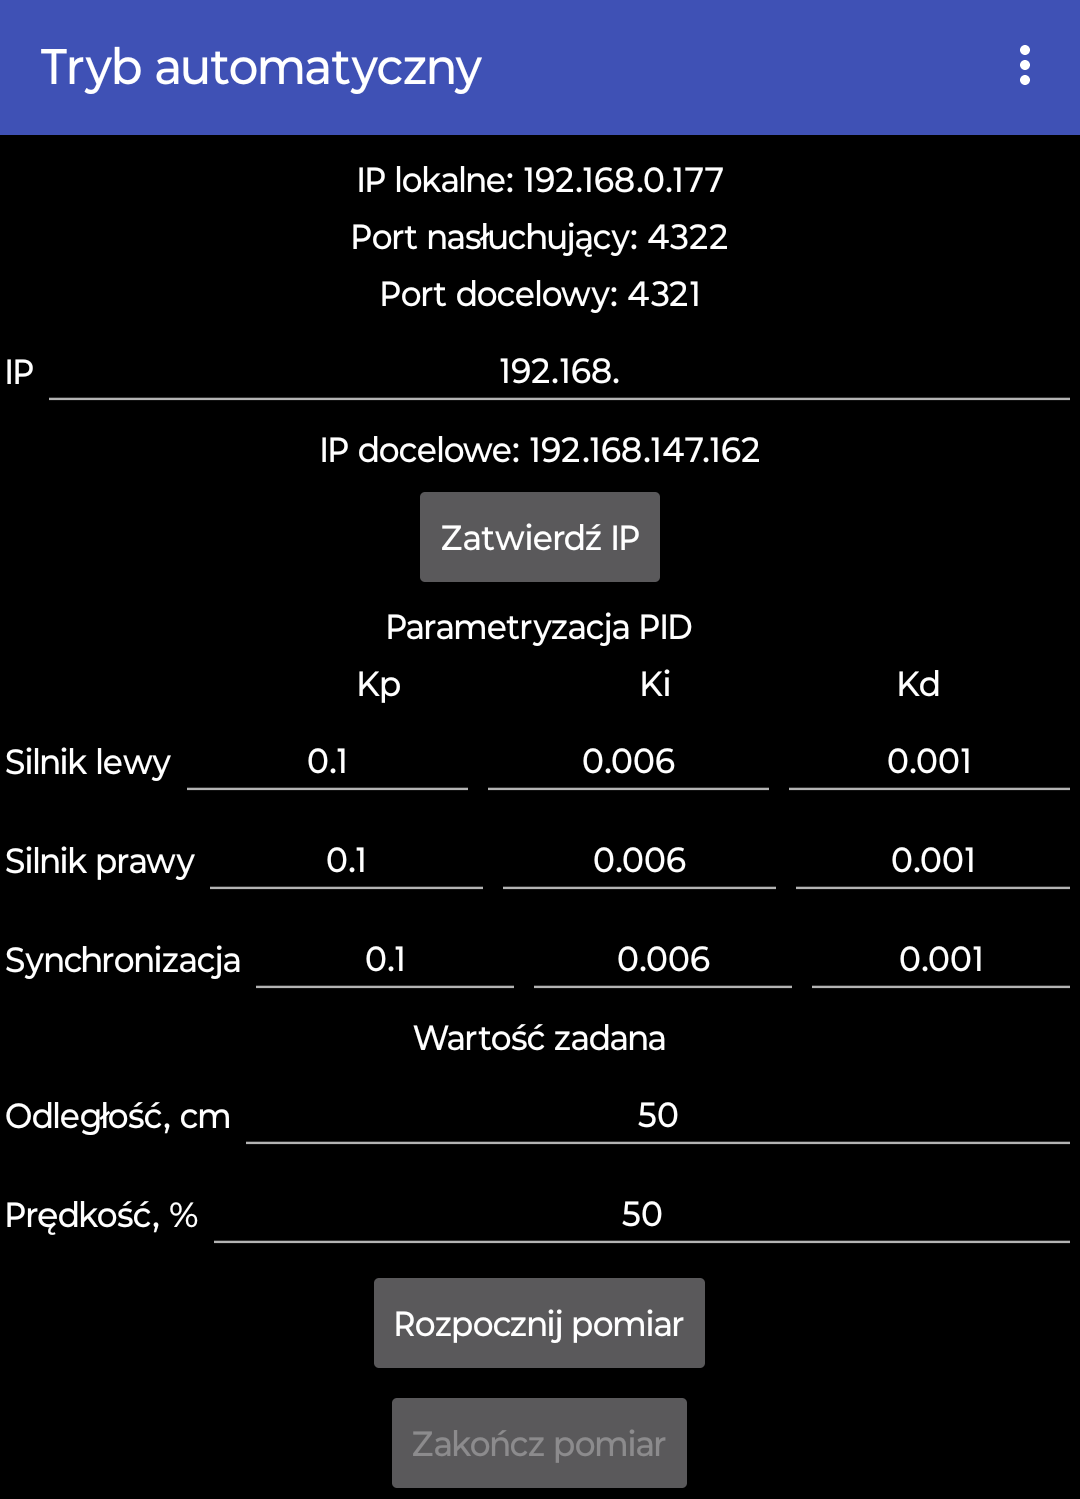
\includegraphics[scale=0.3]{images/AndroidApp.png}
  \captionof{figure}{Zrzut ekranu aplikacji sterującej}
  \label{fig:aplikacja}
\end{center}

\subsection*{Skrypt Python}
Krótki skrypt działający w pętli --- na początku tworzy pusty plik .csv, następnie oczekuje na pomiar. Po otrzymaniu danych pomiarowych i~zapisaniu ich do utworzonego pliku .csv, oczekuje na interakcję użytkownika. W~tym momencie można skopiować otrzymane dane poprzez skopiowanie pliku lub zmianę jego nazwy. Na komendę użytkownika, skrypt czyści plik .csv i~pętla zaczyna się od nowa. Wadą skryptu jest brak możliwości zakończenia go innej, niż zamknięcie procesu. Plik .csv zawiera

\subsection*{Skrypt MATLAB}
Mimo nazwy podrozdziału, skrypty w~MATLABie są ostatecznie dwa, nie jeden, choć pełnią podobne funkcje. Rozdzielone zostały dla czystości i~wygody użytkowania. Pierwszy z~nich wykreśla charakterystykę statyczną, będącą funkcją zależności pulsów na pętlę od prędkości w~biegu jałowym. Szczegółowy opis znajduje się w~Rozdziale~\ref{ch:experiment}. Robi to odczytując pomiary z~zakresu prędkości $\left<0; 100\right>$, ze skokiem równym 5\%,~a~następnie na ich podstawie rysując i~łącząc punkty.

Drugi skrypt wykreśla 3~wykresy. Pierwszym jest pozycja silników, wyrażona w~funkcji zależności pozycji silników od czasu. Drugi pokazuje zadaną w~danym momencie przez regulatory PID wartość prędkości zadanej w~procentach. Innymi słowy, jest to wykres zależności prędkości zadanej (w procentach) silników od czasu. Trzeci przedstawia prędkość rzeczywistą silników w~postaci funkcji zależności rzeczywistej prędkości silników (w~pulsach na pętlę) od czasu. Na każdym wykresie ukazane są 2~funkcje, po jednej na silnik.